\documentclass[12pt,a4paper]{report}

\usepackage[utf8]{inputenc} % pentru suport diacritice
\usepackage[romanian]{babel} % setări pentru limba română
\renewcommand\familydefault{\sfdefault} % sans serif

\usepackage[margin=2.54cm]{geometry}	% dimensiuni pagină și margini
\usepackage{graphicx} % support the \includegraphics command and options

% formatting sections and subsections
\usepackage{textcase}
\usepackage[titletoc, title]{appendix}
\usepackage{titlesec}
\titleformat{\chapter}{\large\bfseries\MakeUppercase}{\thechapter}{2ex}{}[\vspace*{-1.5cm}]
\titleformat*{\section}{\large\bfseries}
\titleformat*{\subsection}{\large\bfseries}
\titleformat*{\subsubsection}{\large\bfseries}

\usepackage{chngcntr}
\counterwithout{figure}{chapter} % no chapter number in figure labels
\counterwithout{table}{chapter} % no chapter number in table labels
\counterwithout{equation}{chapter} % no chapter number in equation labels

\usepackage{booktabs} % for much better looking tables
\usepackage{url} % Useful for inserting web links nicely
\usepackage[bookmarks,unicode,hidelinks]{hyperref}

\usepackage{array} % for better arrays (eg matrices) in maths
\usepackage{paralist} % very flexible & customisable lists (eg. enumerate/itemize, etc.)
\usepackage{verbatim} % adds environment for commenting out blocks of text & for better verbatim
\usepackage{subfig} % make it possible to include more than one captioned figure/table in a single float
\usepackage{enumitem}
\setlist{noitemsep}

%%% HEADERS & FOOTERS
\usepackage{fancyhdr}
\pagestyle{empty}
\renewcommand{\headrulewidth}{0pt}
\renewcommand{\footrulewidth}{0pt}
\lhead{}\chead{}\rhead{}
\lfoot{}\cfoot{\thepage}\rfoot{}

\newcommand{\HeaderLineSpace}{-0.25cm}
\newcommand{\UniTextRO}{UNIVERSITATEA POLITEHNICA DIN BUCUREȘTI \\[\HeaderLineSpace]
FACULTATEA DE AUTOMATICĂ ȘI CALCULATOARE \\[\HeaderLineSpace]
DEPARTAMENTUL DE CALCULATOARE\\}
\newcommand{\DiplomaRO}{PROIECT DE DIPLOMĂ}
\newcommand{\AdvisorRO}{Coordonator științific:}
\newcommand{\BucRO}{BUCUREȘTI}

\newcommand{\UniTextEN}{UNIVERSITY POLITEHNICA OF BUCHAREST \\[\HeaderLineSpace]
FACULTY OF AUTOMATIC CONTROL AND COMPUTERS \\[\HeaderLineSpace]
COMPUTER SCIENCE AND ENGINEERING DEPARTMENT\\}
\newcommand{\DiplomaEN}{DIPLOMA PROJECT}
\newcommand{\AdvisorEN}{Thesis advisor:}
\newcommand{\BucEN}{BUCHAREST}

\newcommand{\frontPage}[6]{
\begin{titlepage}
\begin{center}
{\Large #1}  % header (university, faculty, department)
\vspace{50pt}
\begin{tabular}{p{6cm}p{4cm}}

\includegraphics[scale=0.8]{pics/upb-logo.jpg} &
	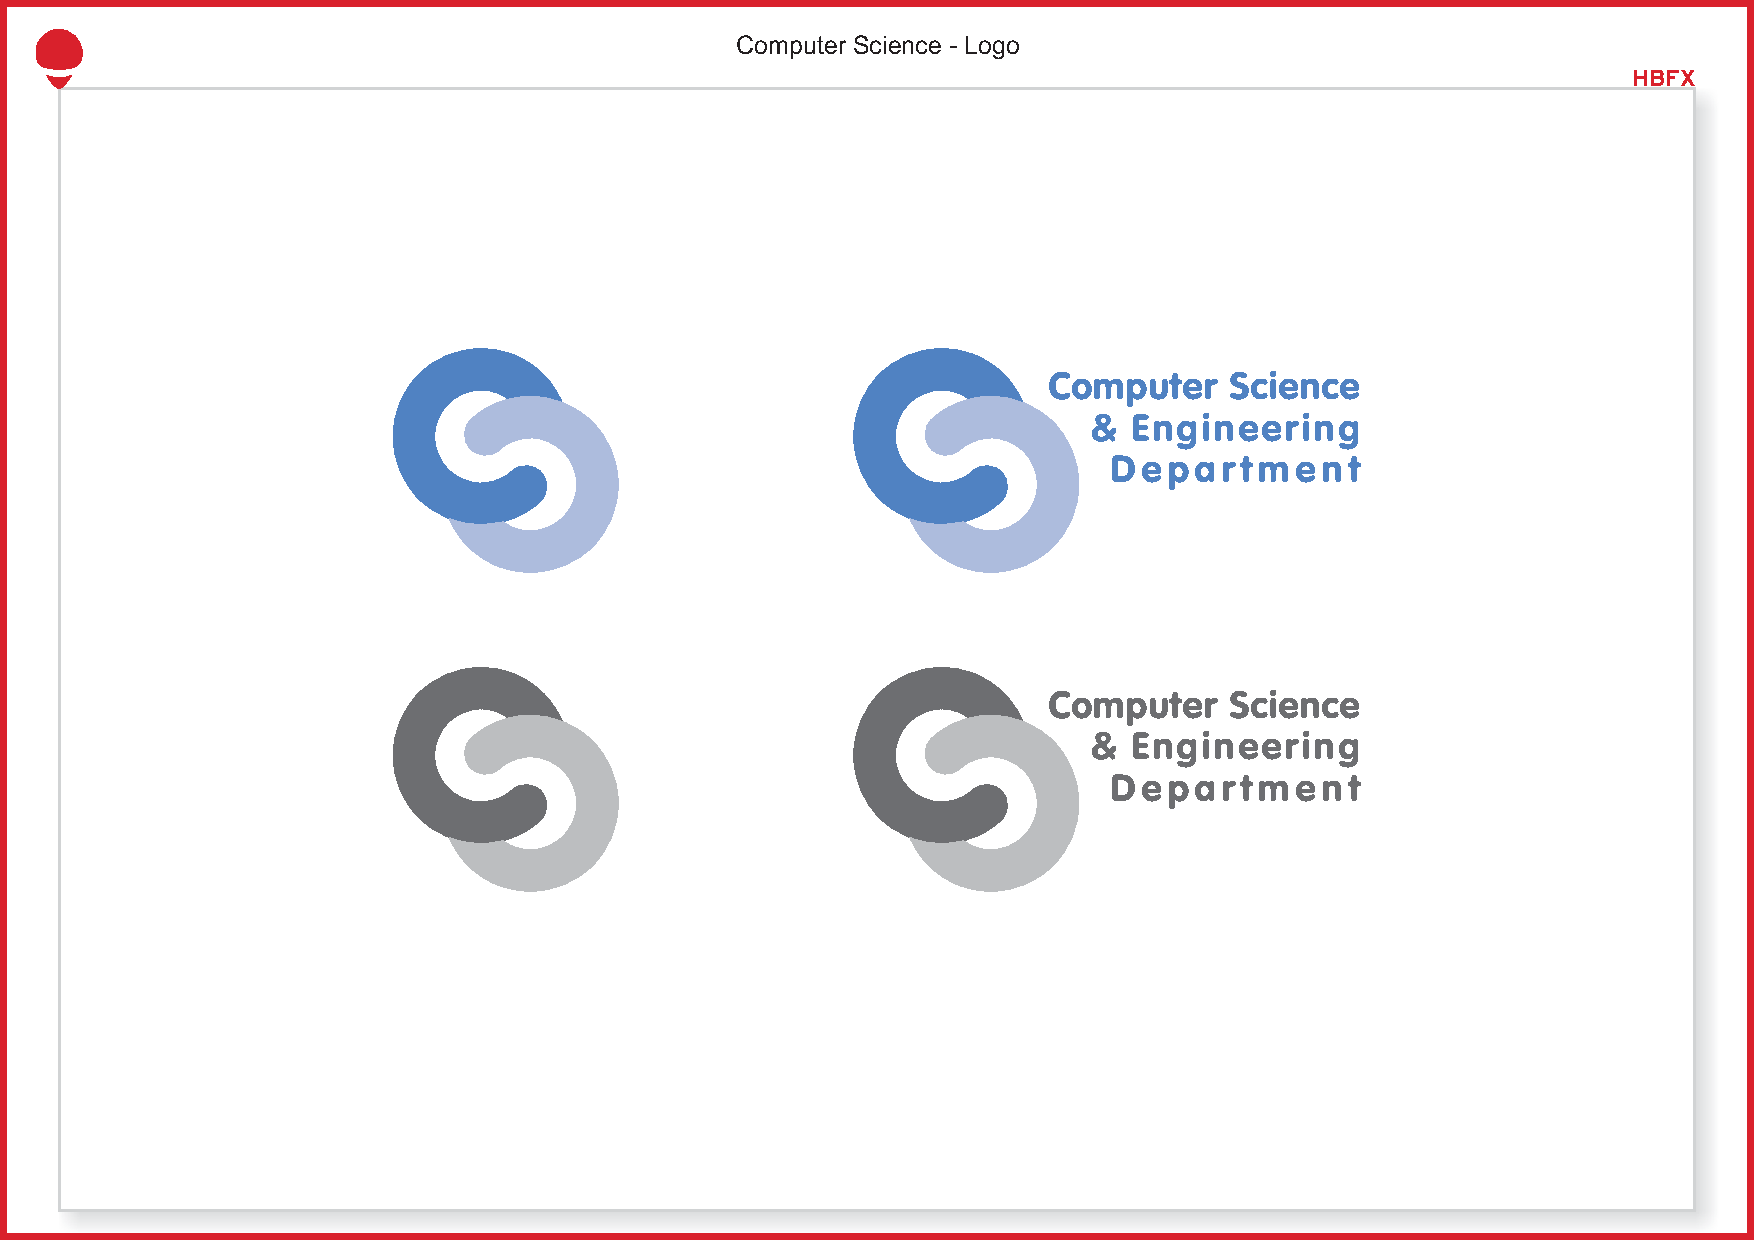
\includegraphics[scale=0.5,trim={14cm 11cm 2cm 5cm},clip=true]{pics/cs-logo.pdf}
\end{tabular}

\vspace{105pt}
{\Huge #2}\\                           % diploma project text
\vspace{40pt}
{\Large #3}\\ \vspace{0pt}  % project title
{\Large #4}\\                          % project subtitle
\vspace{40pt}
{\LARGE \Name}\\                   % student name
\end{center}
\vspace{60pt}
\begin{tabular*}{\textwidth}{@{\extracolsep{\fill}}p{6cm}r}
&{\large\textbf{#5}}\vspace{10pt}\\      % scientific advisor
&{\large \Advisor}                                    % advisor name
\end{tabular*}
\vspace{20pt}
\begin{center}
{\large\textbf{#6}}\\                                % bucharest
\vspace{0pt}
{\normalsize \Year}
\end{center}
\end{titlepage}
}

\newcommand{\frontPageRO}{\frontPage{\UniTextRO}{\DiplomaRO}{\ProjectTitleRO}{\ProjectSubtitleRO}{\AdvisorRO}{\BucRO}}
\newcommand{\frontPageEN}{\frontPage{\UniTextEN}{\DiplomaEN}{\ProjectTitleEN}{\ProjectSubtitleEN}{\AdvisorEN}{\BucEN}}

\linespread{1.15}
\setlength\parindent{0pt}
\setlength\parskip{.28cm}

%% Abstract macro
\newcommand{\AbstractPage}{
\begin{titlepage}
\textbf{\large SINOPSIS}\par
\AbstractRO\par\vfill
\textbf{\large ABSTRACT}\par
\AbstractEN \vfill
\end{titlepage}
}

%% Thank you macro
\newcommand{\ThanksPage}{
\begin{titlepage}
{\noindent \large\textbf{MULȚUMIRI}}\\
\Thanks
\end{titlepage}
}



%%%%%%%%%%%%%%%%%%%%%%%%%%%%%%%%%%%%%%%%%%%%%%%%%%
%%
%%          End of template definitions
%%
%%%%%%%%%%%%%%%%%%%%%%%%%%%%%%%%%%%%%%%%%%%%%%%%%%


%%% Puteți elimina aceste linii din lucrare, servesc numai pentru template.
\newcommand{\worktype}[1]{[\textit{#1}] }
\newcommand{\dezvoltare}{\worktype{Dezvoltare de produs}}
\newcommand{\cercetare}{\worktype{Cercetare}}
\newcommand{\ambele}{\worktype{Ambele}}
%%%


%%
%%   Campurile de mai jos trebuie modificate de autor. Modificati doar continutul, nu si numele fiecarei definitii
%%
\newcommand{\ProjectTitleRO}{Portarea infrastructurii de testare IxOS pe SBC-uri ARM}
\newcommand{\ProjectSubtitleRO}{~ }
\newcommand{\ProjectTitleEN}{Porting IxOS testing infrastructure on ARM SBCs}
\newcommand{\ProjectSubtitleEN}{~ }
\newcommand{\Name}{Lucian-Ioan Popescu}
\newcommand{\Advisor}{Dr. ing. Lucian Mogosanu}
\newcommand{\Year}{2022}

% Setări document
\title{Proiect de diplomă}
\author{\Name}
\date{\Year}

%%
%%   Campurile aferente rezumatului
%%
\newcommand{\AbstractRO}{

Pana in prezent portarea se bazeaza pe metode ad-hoc care au la baza factori ca experienta
dezvoltatorului sau claritatea sistemului ce se vrea portat. Acest studiu ofera o prezentare a
problemei portarii software bazandu-ne pe experienta practica de a porta infrastructura de testare Ixia
pe arhitectura ARM. Pentru acomodarea pe noua platforma am facut modificari ce tin de interfatarea
cu sistemul de operare sau de pastrarea compatibilitatii cu celelalte componente ale ecosistemului.
Testarea s-a desfasurat in mai trei etape: etapa functionala, etapa de performanta si
evaluarea procesului de portare. Rezultatele arata ca TBD. Aceste rezutlate faciliteaza formalizarea
unor tehnici de portare explicate pe larg de-a lungul lucrarii, cum ar fi impartirea si decuplarea
unitatilor sistemului sau izolarea bucatilor dependente de arhitectura.

}

\newcommand{\AbstractEN}{
TBD
}


%%
%%   Campurile aferente paginii de multumiri
%%
\newcommand{\Thanks}{(opțional) Aici puteți introduce o secțiunea specială de mulțumiri / acknowledgments. }

\begin{document}

\frontPageRO
\frontPageEN

\begingroup
\linespread{1}
\tableofcontents
\endgroup

\AbstractPage

% poate fi comentata sau stearsa
\ThanksPage


% Textul licentei incepe de aici



\chapter{Introducere}\pagestyle{fancy}
% * <marios.choudary@gmail.com> 2018-02-28T11:38:18.106Z:
%
% > INTRODUCERE
% Am scos de aici referintele la font pentru a nu mai fi dependenti de Calibri. Personal, nici nu sunt sigur ca ajuta prea mult aceasta recomandare si mi se pare bun font-ul default din Latex (Computer Modern). Daca sunteti de-acord, va rog sa stergeti liniile comentate de mai jos, precum si cele referitoare la fontul Calibri din restul documentului.
%
% ^.
There are many reasons why developers port code from one architecture to another. These reasons
include performance enhancements, deprecation of old hardware or trying to make use of features
that are available only on a specific architecture. Frakes et al~\cite{frakes1995sixteen} discovered
that the persons involved in the developing process prefer to reuse code instead of build it from
scratch. This happens because the effort of porting an existing piece of code is often lower than
the effort of writing it from the ground up. This is true especially in the enterprise environment
where people try to patch different systems together in order to have a fast deliverable~\cite{rettig2007trouble}.

Software development costs and invested resources are big. We would like to preserve these
investments when the need for a new architecture arises. To achieve this goal people designed
programming languages and compilers that increased portability, operating systems that could run
on multiple hardware platforms~\cite{johnson1978unix} and various standards that allowed developers
to talk to the computer using well defined interfaces~\cite{walli1995posix}. However the porting
process is a non-trivial endeavor up to this day, it is error prone and badly formalized. The
happens because the initial architecture contains implicit assumptions about the environment as:
endianess, non-standard compiler behavior or custom changes made in the operating system structure;
or it may happen because the developers make use of non-portable constructs as ifdefs
\cite{spencer1992ifdef} or machine dependant code. Moreover these parts of the design and
environment are recorded in human-readable documents that are hard to preserve over time or the
information is not recorded at all. Thus forcing the developer to rely on its own experience and
skills in order to solve the porting problems that will arise.

Ghandorh et al~\cite{ghandorh2020systematic} discovered that the porting process relies on ad-hoc
techniques. Their work presents an unified testing framework for assuring the quality of porting
a system from one architecture to another. However this does not solve the whole problem as there
is no standardized process of describing the work of porting per se. Each system has its own
peculiarities as discussed above, making the standardization process hard to formulate. In this
paper we try to propose such a standard in order to minimize the efforts and increase the
productivity of the developers.

To succesfully complete this task, we describe the experience of porting the existing Ixia testing
infrastructure, IxOS, on ARM devices. Currently it is implemented for x86, MIPS and PowerPC. The
porting involved multiple stages of planning and execution because the system was heavily rooted
in its ecosystem, making it hard for us to decouple the desired components. From build system to
interaction with the other components, IxOS proved itself hard to port because problems and errors
arose out of nowhere. For example the compilation toolchain had missing macro definition that needed
to be manually solved, bugs appeared in system libraries because we compiled the code on a new
hardware architecture and specific zones of logic needed to be hardcoded in order to keep
compatibility with the ecosystem. However we successfully ported the code on the ARM device of our
choice, Raspberry Pi 4.

To evaluate our porting results we chose three types of testing:
\begin{itemize}
	\item functional testing. We assured using manual testing that the main features of the
		system were well preserved on the new architecture.
	\item porting testing. The quality of the porting process was measured using techniques
		described in Ghandorh et al~\cite{ghandorh2020systematic}. Some of these techniques
		include measurements as environment independecnce, degree of portability or porting
		costs.
	\item performance testing. Using this method we tried to understand if the system behaves
		better or werse than the old architecture in terms of memory consumption, cpu load
		and total time spend in intensive areas.
\end{itemize}

In this work we make the following contributions. First, we conduct a comprehensive study on the
porting process of systems to various architectures, identifying common difficulties,
inconsistencies and best practices. Second, we expose the experience of porting a large scale
enterprise project as IxOS on an ARM off-the-shelf board, Raspberry Pi. By doing this we focus on
the difference between accidental and essential tasks as described by Brooks et al~\cite{brooks1987no},
i.e. the difference between porting and portability. Third, we propose a
standardized recipe for porting a system to a new architecture and discuss about the requirements
for obtaining maximum efficiency for this recipe. The discussion inclueds topics as the
importance of documentation, efficient methods for documenting ideas and system architecture designs
that maximize portability.

The rest of this work is organized as follows. Section 2 and 3 discuss the background and related
work with regards to portability. Section 4 discusses the previous work done inside Keysight that
facilitated the completion of our porting experiment. Section 5 described the porting of IxOS
infrastructure on Raspberry Pi. Section 6 explores how the porting process and porting results were
evaluated. Section 7 gives a retrospective on our work and formalized the porting process. Section
8 presents a conclusion to this work and enumerates the future work.

\chapter{Background and Related Work}

\section{Background}

While developing complex software, developers tend to focus on writing code for a given set of
requirements. These requirements, however, need adaptation as they change throughout the life
of the software project. Thus, software code must also adapt to the new requirements. When the
adaptation process consists of a change in the software or hardware environment, it is called
porting process, from the Latin \textit{portare}. i.e. "to carry"~\cite{etymology}.

In general, a software process is a sequence of activities that lead to the production of a software system
when executed~\cite{humphrey1995discipline}. These processes can be observed in all kinds of
software development settings, allowing people who use them to have a well defined set of
expectations and results after implementing the respective process. Porting can be regarded as a
software process, making possible for the developers to decide if the practice of porting a software
system can be improved by investing more resources as human power or automated software analysis
tools, or by making modifications to the current implementation, for example choosing to refactor
software units to make porting more manageable.

In particular, porting is the act of producing an executable version of a software unit or system in a new
environment based on an existing version~\cite{mooney1993issues}. This is seldom an easy task
because it involves a good amount of code rafactoring and architectural redesign. It can be
avoided, however, if the original design has portability incorporated by using constructs as
multi-platform libraries, modular code or standard compiler behaviors.

Mooney~\cite{mooney1993issues} presents two components of the porting process: transporation and
adaptation. The first is described as the act of moving the system (code or binary executable) to a
new environment and the latter is described as the act of modifying the system in order to be
compatible with the new environment. Transportation is facilitated by communication channels
to the target environment, either online (file sharing systems, remote connections) or physical
(using data storage devices). If transportation can be neglected, adaptation is more developement
resources consuming because it implies translating the source code to the new architecture, solving
possible inconsistencies and making sure that the software system behaves in a well defined manner
when ran in the new environment.

The environment is defined as the
set of software and hardware elements that interact with the system. This includes, but it is not
restricted to: operating system, communication methods, configuration files and system variables,
hardware architecture or human interaction. Two software environments involved in the porting
process will never be the same because of the software and hardware inconsistencies. On one hand,
programs between operating systems will not work, even if the hardware is the same. For example MacOS
uses MACH for executable files while Linux uses ELF, moreover even if they follow the POSIX
standard, they may have implementation details that do not align with each other. On the other
hand, processor architectures vary from one another in the way they understand machine language
and even if they do not vary, custom hardware attached to these processors makes porting difficult as
the software must be rewritten in order to accomodate the new periferials.

Portability referes to the ability of software to be ported to another
environment. In the real world, a software unit or system can never be fully portable because the
environments have their own peculiarities. Even though standards help in situations as this one,
they cannot solve the whole problem of zero-cost portability. This happens because each standard
focuses on specific requirements that the standardized system must meet. For example POSIX
(ISO/IEC 9945-1) was designed to ease the task of cross-platform software development by
establishing a set of guidelines for operating system vendors to follow. On the other hand CTRON
standard~\cite{wasano1989application} was designed for common application to network nodes, whether
for switching, communications
processing, or information processing, and is aimed at improved portability through realtime
performance and fault tolerance. The two standards clearly share a common ground, namely portability,
but also differ in subtle manners (CTRON is designed for network communicaton, while POSIX is more
generic). An universal standard that combines POSIX and CTRON would indeed create a more approachable
solution for the zero-cost portability problem but would limit the intrinsic expressiveness of
each standard. Because of these differences between environments, it is more accurate to characterize
software through a degree of porability, instead of simply saying that a software system is either
portable or not.

The degree of portability is directly characterized by the cost of porting (CP) and the cost of
redevelopment (CD). If CP is greater than CD then porting is more costly and should be avoided,
otherwise porting is the preferred solution. This metric is mostly useful when the developers are
given a software unit and a new environment, so that they must decide whether is more favorable
to port the software unit or to rewrite it for the new environment. However the cost of porting
and cost of redevelopment are generic notions that must be deeply analyzed in order to achieve
clear results. This analysis is highly dependent on each software project and must consider
factors as: experience of developers, quality of code and documentation or software units
complexity.

When introducing portability as a requirement in a software project, one must carefully analyze all
the aspects of the different environments that will operate with the project. Some of the most
important aspects are: CPU architectures, operating systems, compilers and build environments.
The next paragraph presents some questions the developer must respond in order to provide a high
degree of portability with regards to the above aspects.

The differences underlying the CPU architecture expose themselves in many ways to developers, from
word size and word order to word alignment. What is the size of primitive data types as: char, int
or long? Which type of binary arithmetic is used? Are there peculiarities regrading data type
pointers or function pointers? Exotic machines as Unisys 1100/2200 have 9 bit chars
and 36 bit ints and longs, using ones' complement binary logic, pointers that cannot be treated
as integers and function pointers that are 8 words long.
Operating systems also have major limitations
in terms of portability. One must answer the following questions to
find out whether the software project is portable: Are threads supported, which semantics do threads
use? How is process management and interprocess communication achieved? Is device I/O control
possible? For example, device I/O control in Windows is achieved through DeviceIoControl~\cite{grantmestrength}
while Unix systems use ioctl~\cite{ioctl_linux, ioctl_openbsd, ioctl_freebsd}.
Compiler portability can also become problematic as not all compilers accept the same language.
Should I use preprocessor
flags in order to accomodate multiple semantics of different compilers? Are there any differences
between the code generated by two compilers for the same unit of code?
What are the constructs specific only to this type or version of compiler? For example, clang and GCC
do not support the same C language in terms of C99 inline functions, vector builtin functions,
lvalue casts, \_\_block variables and inline assembly~\cite{language_compatibility}.
The build environment is the set of all software and tools required to go from source code to any
form of final product. This includes compiler, linker, third-party libraries, a build tool and
configuration scripts. However the usage of the above mentioned components is not portable across
different environments. Does the environment support interpretors for running the configuration
scripts? Are the third-party libraries portable to run on this environment? What is the proper way
to enable all warnings on this compiler? Are dynamic libraries supported and what semantics do they use?
For example, to load a shared library the developer can use dlopen on POSIX systems, shl\_load on
HP-UX or NSAddImage or NSLinkModule on Darwin and Mac OS X.

In this section, we presented the anatomy of porting as a software process using building blocks
as environment dependencies, transportation and adapatation of code. Moreover, we presented
portability as a quality of software systems that decides whether the software system can be
ported or not using concepts as degree of portability and in-depth dependencies as CPU architecture
or compilers.

\section{Related Work}

TODO

% Asa se specifica folosirea unui fisier cu referinte bibliografice:
\bibliographystyle{plain}
\bibliography{bibliography}

%% O alta varianta ar fi fost includerea de articole direct in acest fisier
%% in felul urmator:
%% \begin{thebibliography}{ABC}
%%
%% \bibitem{article}
%%  H. Baali, H. Djelouat, A. Amira and F. Bensaali,
%%  ``Empowering Technology Enabled Care Using IoT and Smart Devices:
%   A Review''. In: IEEE Sensors Journal, vol. 322 (10), pp. 891--921, 1905.
%%
%% (more \bibitem items here...)
%%
%% \end{thebibliography}

%% Daca vreti ca o sectiune sa inceapa pe o pagina noua, puteti forta acest lucru cu comanda "\newpage", ca mai jos:

%\newpage

\chapter*{Anexe}\addcontentsline{toc}{chapter}{Anexe}

Anexele sunt opționale.
Ce poate intra în anexe:
\begin{itemize}
\item	Exemplu de fișier de configurare sau compilare;
\item	Un tabel mai mare de o jumătate pagină;
\item	O figura mai mare mai mare de jumătate pagină;
\item	O secvență de cod sursa mai mare de jumătate pagină;
\item	Un set de capturi de ecran (``screenshot''-uri);
\item	Un exemplu de rulare a unor comenzi plus rezultatul (``output''-ul) acestora;
\item 	În anexe intră lucruri care ocupă mai mult de o pagină ce ar întrerupe firul natural de parcurgere al textului.
\end{itemize}

\begin{appendices}

\chapter{Extrase de cod} % Introduce o nouă anexă
\ldots


\end{appendices}
\end{document}
